\clearpage
\title{Problem 6.2}
\author{}
\date{}
\maketitle

\section*{Problem Description}
Write a code to take input from user as string and then out the string in reverse. Use stack.

\section*{Process}
\subsection*{Code:}

\begin{multicols}{2}{|}
    \begin{minted}[linenos,breaklines,breakanywhere]{nasm}
DATA SEGMENT

DATA ENDS
CODE SEGMENT
    ASSUME CS:CODE, DS:DATA
    
START:
    MOV AX, DATA
    MOV DS, AX
    
    XOR CX, CX
    MOV AH, 1
    INT 21H
    
INPUT:
    CMP AL, 0DH
    JE EXIT_
    
    PUSH AX
    INC CX
    
    INT 21H
    JMP INPUT     
    
EXIT_:   
    MOV AH, 2
    MOV DL, 0DH
    INT 21H
    MOV DL, 0AH
    INT 21H
    
OUTPUT:
    POP DX
    INT 21H
    LOOP OUTPUT
     
CODE ENDS
END START  
\end{minted}
\end{multicols}

\subsection*{Output}
\begin{center}
    \centering
    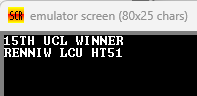
\includegraphics[width = .4\textwidth]{stkRev.png}
    \captionof{figure}{Hexadecimal input \& output}
\end{center}


